\documentclass{article}

\usepackage[main, final]{neurips_2026}
\usepackage[utf8]{inputenc}
\usepackage[T1]{fontenc}
\usepackage{hyperref}
\usepackage{url}
\usepackage{booktabs}
\usepackage{graphicx}
\usepackage{microtype}
\usepackage{xcolor}

\graphicspath{{./}{report/Group_report/}}

\title{Daily arXiv Research Briefing Agent}

\author{%
  Group Report \\
  Yanzhe Xie, Che Feng \\
  Social Network Analysis, Spring 2026
}

\begin{document}

\maketitle

\begin{abstract}
The Daily arXiv Research Briefing Agent is a local Agent and Skills system for personalized paper discovery. Given a topic, an optional arXiv category, a date range, seed papers, feedback, or a follow-up query, the Agent retrieves candidate papers, ranks them using topic, seed, semantic, and feedback signals, and produces an evidence-aware daily briefing. The system represents papers, topics, categories, seed preferences, retrieval runs, and feedback events as an academic information network. The Agent integrates two independently testable public Skills. DiscoveryRecommendationSkill supports query planning, retrieval, recommendation, feedback refinement, and local-first follow-up filtering. ResearchSynthesisSkill supports structured paper extraction, briefing generation, and selected-paper explanation. A shared SQLite layer stores metadata, retrieval runs, seed preferences, feedback events, full-text cache rows, and embedding cache rows. Fixture-based evaluation achieves precision@3, recall@3, MRR, rationale coverage, required-section coverage, and Top-K briefing coverage of 1.0. A frozen real-arXiv ranking study further compares deterministic ranking, semantic ranking, and BM25.
\end{abstract}

\section{Functionality}

Researchers face a persistent filtering problem because arXiv publishes more papers each day than a user can inspect manually. This project converts a compact research interest into a ranked reading list, a structured daily briefing, and follow-up explanations with explicit evidence labels. The Agent represents topics, arXiv categories, papers, seed papers, user profiles, feedback events, and recommendation rationales as linked elements in an academic information network. Edges encode retrieval provenance, topical overlap, seed-paper similarity, feedback preference, and synthesis evidence. This design satisfies the course requirement for an Agent and Skills system: independent modules communicate through structured data, and the orchestrator composes them into a single workflow.

The main entry point is DailyArxivAgentOrchestrator. It accepts requests from the command line interface or the Streamlit user interface and supports topic keywords, arXiv category, submitted-date range, Top-K size, seed papers, profile preferences, feedback, follow-up queries, selected-paper explanation mode, and provider configuration. Its output is a RecommendationWorkflow that contains candidate papers, ranked recommendations, extracted briefing items, the final daily briefing, and a workflow trace. Each trace step records status, evidence source, fallback state, input and output summaries, and structured errors.

The user-facing outputs cover three workflows. The Agent generates a daily briefing with an executive summary, a summary table, a highlighted paper, Top-K paper notes, comparisons, reading priorities, and an evidence boundary. It records feedback and returns a refined ranking with rank and score changes. It also supports local-first follow-up filtering.

\begin{figure}[t]
  \centering
  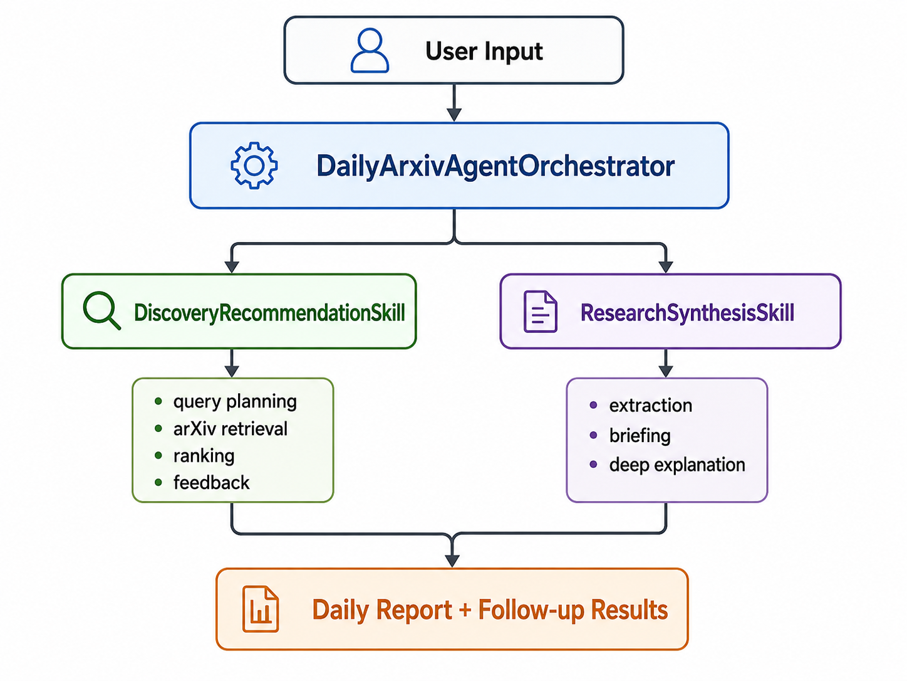
\includegraphics[width=0.92\linewidth]{overview.png}
  \caption{Agent architecture. DailyArxivAgentOrchestrator coordinates two public Skills through structured contracts and a shared SQLite state layer. DiscoveryRecommendationSkill handles query planning, retrieval, ranking, feedback, and follow-up. ResearchSynthesisSkill handles extraction, briefing, and selected-paper explanation.}
  \label{fig:agent-architecture}
\end{figure}

\section{Agent Design}

Figure~\ref{fig:agent-architecture} shows the implemented architecture. The orchestrator coordinates Skills, records workflow traces, and preserves the shared result contract. DiscoveryRecommendationSkill wraps seed parsing, query planning, arXiv retrieval, deterministic ranking, semantic seed ranking, feedback refinement, and follow-up filtering. ResearchSynthesisSkill wraps per-paper extraction, daily briefing generation, and selected-paper deep explanation. Older fine-grained Skills remain available internally, which keeps evaluation precise while presenting the deliverable as an Agent with two public Skill boundaries.

The workflow begins by building a RetrievalQuery. When seed papers are provided, SeedParsingSkill converts arXiv IDs, arXiv URLs, or titles into a SeedPreference. QueryPlanningSkill creates a QueryPlan with required terms, optional terms, phrases, categories, and query variants. Invalid LLM-assisted plans fall back to deterministic planning before retrieval. ArxivRetrievalSkill calls the arXiv Atom API when needed, parses metadata, and caches normalized PaperMetadata records in SQLite.

Ranking follows two paths. The deterministic path combines topic matches, query-plan terms, phrases, category and date context, seed preference text, retrieval provenance, and feedback events. The semantic seed path checks embedding readiness, fails closed when the configuration is unsafe, and otherwise compares seed and candidate embeddings while retaining lexical, category, and recency signals. Both paths score edges between user intent nodes and paper nodes, and both output Recommendation rows with rank, score, rationale, evidence source, and score breakdown.

ResearchSynthesisSkill consumes the Top-K recommendations rather than retrieving or reranking papers. PaperExtractionSkill creates PaperBriefingItem records with summaries, contribution claims, method cues, relevance rationales, and reading guidance. DailyBriefingSkill combines those items with candidate-pool, query-plan, retrieval, and ranking context. PaperDeepExplanationSkill supports method, experiment, and limitations modes. It prefers full text when available and then falls back to abstracts or metadata with explicit labels, preventing weak evidence from being presented as full-paper analysis.

SQLitePaperStore stores paper metadata, retrieval runs, seed preferences, feedback events, full-text cache rows, and embedding cache rows. This shared layer keeps the two public Skills independent. All public methods return SkillResult objects with success, empty, fallback, or error status, so the CLI, UI, tests, and report apply the same interpretation to outputs and failure cases.

\section{Related Work}

The project builds on scholarly information retrieval, recommender systems, semantic similarity, and evidence-grounded generation. arXiv metadata access follows the arXiv API \citep{arxivapi}. The recommendation design follows ranked retrieval practice by reporting precision, recall, and mean reciprocal rank, and by separating candidate generation from ranking \citep{manning2008}. It also follows hybrid recommender-system ideas, in which topic, category, content, seed papers, and user feedback provide complementary signals \citep{burke2002}. Semantic seed ranking follows sentence embedding similarity, where related texts are represented in a vector space so that seed papers can personalize ranking beyond exact keyword overlap \citep{reimers2019}. The academic information network gives these signals a common representation.

The synthesis component follows retrieval-augmented generation, where generated text is conditioned on retrieved evidence and exposes the boundary between source material and generation \citep{lewis2020}. Research on faithfulness in summarization shows that fluent summaries may contain unsupported claims, so the Agent treats evidence labels and abstentions as part of the output contract \citep{maynez2020}.

\section{Results}

Evaluation uses deterministic fixtures and helper metrics in daily\_arxiv\_agent.evaluation.metrics. The goal is to verify reproducibility, output coverage, measurable ranking and feedback effects, and evidence discipline, rather than to claim state-of-the-art recommendation quality. The main search-quality fixture contains exact, related, weak, and unrelated candidates for multimodal LLM agents for robotic manipulation. A frozen real-arXiv ranking set adds three topics, 150 recent candidates, binary human relevance labels, and BM25 comparisons.

\begin{table}[t]
  \centering
  \caption{Group-level evaluation. Fixture rows measure reproducible workflow behavior, and real-arXiv rows report macro averages over three frozen topics and 150 candidates.}
  \label{tab:group-results}
  \small
  \begin{tabular}{@{}p{0.25\linewidth}p{0.47\linewidth}p{0.20\linewidth}@{}}
    \toprule
    Evaluation area & Metric & Result \\
    \midrule
    Search quality & relevant candidate coverage & 1.0 \\
    Recommendation & precision@3 / recall@3 / MRR & 1.0 / 1.0 / 1.0 \\
    Ranking explainability & rationale coverage & 1.0 \\
    Daily briefing & required-section coverage & 1.0 \\
    Daily briefing & Top-K coverage & 1.0 \\
    Daily briefing & forbidden full-text claims & none \\
    Deep explanation & method-mode completeness & 0.86 \\
    Real-arXiv short topics & best precision@5 / recall@10 & 0.800 / 0.944 \\
    Real-arXiv intent topics & semantic precision@5 / recall@10 & 0.733 / 0.722 \\
    \bottomrule
  \end{tabular}
\end{table}

Table~\ref{tab:group-results} summarizes the main results. Broad planned search reaches relevant candidate coverage of 1.0 and ranks the three expected relevant papers in Top-K, yielding precision@3, recall@3, and MRR of 1.0. Rationale coverage of 1.0 indicates that every recommendation includes an inspectable explanation. The briefing evaluator reports required-section and Top-K coverage of 1.0 and rejects forbidden full-text claims. The method-mode explanation score is 0.86 because the fixture intentionally omits one required method field. In the frozen real-arXiv study, BM25 gives the strongest short-topic precision@5 and recall@10, while Semantic Agent gives stronger intent-topic precision@5 and recall@10 than BM25.

The qualitative demo includes two cases. With a world model topic and seed papers about world action models, recommendations shift toward robotics-oriented world-model papers. With no fresh topic, the stored profile uses saved seeds and feedback to produce recommendations aligned with robotics and deep learning. These cases show that the Agent stores preference signals, connects them to candidate papers through the academic information network, and exposes the effects of those signals on ranking.

\section{Analysis}

\begin{table}[t]
  \centering
  \caption{Quantitative ablation summary. Each row uses deterministic fixtures or trace counters from the implemented workflow.}
  \label{tab:ablations}
  \resizebox{\linewidth}{!}{%
  \begin{tabular}{llll}
    \toprule
    Component & Metric & Baseline & Full setting \\
    \midrule
    Retrieval & relevant candidate coverage & 0.33 strict phrase & 1.0 planned search \\
    Ranking & precision@1 & 0.0 lexical distractor & 1.0 semantic seed \\
    Feedback & moved papers / unchanged papers & 0 / 3 before feedback & 2 / 1 after feedback \\
    Briefing & claim specificity score & $<0.6$ generic summary & $\geq 0.6$ enhanced briefing \\
    Evidence & forbidden full-text claims & $\geq 3$ violating claims & 0 evidence-bounded claims \\
    Explanation & method-section completeness & incomplete field detected & 0.86, with 1 missing field \\
    Follow-up & arXiv requests on local hit & 1 optional fetch path & 0 local-first path \\
    \bottomrule
  \end{tabular}%
  }
\end{table}

Table~\ref{tab:ablations} reports the main ablations. Query planning improves relevant candidate coverage from 0.33 to 1.0 because it searches beyond a brittle strict phrase. Semantic seed ranking changes the top result in the seed-personalization fixture, improving precision@1 from 0.0 to 1.0 when a lexical distractor has high keyword overlap but low semantic similarity. Feedback refinement is measured by rank movement rather than by subjective preference: two papers move and one remains unchanged after feedback. The enhanced briefing passes the specificity gate that generic text fails, and the evidence-boundary check reduces forbidden full-text claims to zero. Local-first follow-up reduces arXiv calls to zero when stored papers already satisfy the query.

Several limitations remain. The fixture metrics validate workflow correctness and evidence discipline rather than general relevance quality across arXiv. The frozen real-arXiv study is broader than the fixtures, but it still covers only three topics and binary relevance labels. Live arXiv retrieval and live LLM calls are nondeterministic because results, provider behavior, and latency can change. Default briefings do not parse PDFs and should not be interpreted as full-paper surveys. A stronger future evaluation should include more human relevance labels, live-provider latency and cost measurements, longitudinal feedback logs, and graph-level measures over the academic information network.

Overall, the Agent satisfies the project requirements. It integrates public Skills into a coherent workflow, defines clear inputs and outputs, reports results and ablations, provides visualization, and preserves the central evidence boundary: users can see which claims come from metadata, abstracts, rankings, candidate-pool context, or full text.

\begin{thebibliography}{9}

\bibitem[arXiv(2026)]{arxivapi}
arXiv.
\newblock arXiv API User Manual.
\newblock \url{https://info.arxiv.org/help/api/index.html}.

\bibitem[Burke(2002)]{burke2002}
Robin Burke.
\newblock Hybrid recommender systems: Survey and experiments.
\newblock \emph{User Modeling and User-Adapted Interaction}, 12:331--370, 2002.

\bibitem[Lewis et~al.(2020)]{lewis2020}
Patrick Lewis, Ethan Perez, Aleksandra Piktus, Fabio Petroni, Vladimir Karpukhin, Naman Goyal, Heinrich Kuettler, Mike Lewis, Wen-tau Yih, Tim Rocktaschel, Sebastian Riedel, and Douwe Kiela.
\newblock Retrieval-augmented generation for knowledge-intensive NLP tasks.
\newblock \emph{NeurIPS}, 2020.

\bibitem[Manning et~al.(2008)]{manning2008}
Christopher D. Manning, Prabhakar Raghavan, and Hinrich Schutze.
\newblock \emph{Introduction to Information Retrieval}.
\newblock Cambridge University Press, 2008.

\bibitem[Maynez et~al.(2020)]{maynez2020}
Joshua Maynez, Shashi Narayan, Bernd Bohnet, and Ryan McDonald.
\newblock On faithfulness and factuality in abstractive summarization.
\newblock \emph{ACL}, 2020.

\bibitem[Reimers and Gurevych(2019)]{reimers2019}
Nils Reimers and Iryna Gurevych.
\newblock Sentence-BERT: Sentence embeddings using Siamese BERT-networks.
\newblock \emph{EMNLP-IJCNLP}, 2019.

\end{thebibliography}

\end{document}
